\documentclass[10pt,a4paper]{article}

\usepackage[utf8]{inputenc}
\usepackage[polish]{babel}
\usepackage[T1]{fontenc}
\usepackage{makecell}
\usepackage{indentfirst}
\usepackage{graphicx}
\usepackage{placeins}

\usepackage{tocloft}
\renewcommand{\cftsecleader}{\cftdotfill{\cftdotsep}}
\usepackage[hidelinks]{hyperref}

\usepackage[explicit]{titlesec}
\titleformat{\section}{\bfseries\large}{\thesection.}{0.5em}{#1}
\titleformat{\subsection}{\bfseries}{\thesubsection.}{0.5em}{#1}

\newcommand{\quotes}[1]{``#1''}

\title{Techniki internetowe \\ \large Dokumentacja wstępna projektu \quotes{TinDox}}
\author{
    \begin{tabular}{p{6em}p{6em}p{6em}p{6em}}
        \makecell{Jakub \\ Mazurkiewicz} &
        \makecell{Damian \\ Piotrowski} &
        \makecell{Anna \\ Pyrka} &
        \makecell{Łukasz \\ Reszka}
    \end{tabular}
}
\date{Semestr 21Z}

\begin{document}
\maketitle
\tableofcontents
\pagebreak

\section{Cel projektu}
Celem projektu jest opracowanie protokołu do wymiany plików przez sieć IPv4. Zakłada się także stworzenie wydajnego serwera oraz klientów na wybrane platformy.

\section{Protokół TDP}

\subsection{Opis}
TDP to protokół komunikacyjny typu serwer--klient wykorzystujący protokół sterowania transmisją (\href{https://en.wikipedia.org/wiki/Transmission_Control_Protocol}{TCP}). Umożliwia dwukierunkowy transfer plików oraz przeglądanie katalogów znajdujących się na zdalnym dysku.

Komunikaty w protokole wymieniane są za pośrednictwem połączenia głównego (na rysunku oznaczonym jako \quotes{Polecenia i odpowiedzi}). Dane są przesyłane za pośrednictwem dodatkowego połączenia TCP (na rysunku oznaczonym jako \quotes{Dane}) tworzonego tylko na potrzeby pobierania i ładowania plików. Po zakończeniu jednej z tych operacji połączenie nie jest od razu zamykane -- może zostać użyte do kolejnych transferów.

\subsection{Słownik pojęć}
\begin{enumerate}
    \item TDP -- TinDox Protocol.
    \item Aktualny katalog -- każdy zalogowany użytkownik posiada przypisany do siebie katalog bieżący, czyli ten, w którym się aktualnie znajduje.
    \item Sól -- krótki, losowo wygenerowany ciąg składający się z wielkich i małych liter alfabetu łacińskiego oraz cyfr, identyfikujący pewną operację lub plik.
    \item Kod operacji -- losowo wygenerowany 32-bitowy kod identyfikujący pewną złożoną operację (np. pobieranie pliku).
\end{enumerate}

\pagebreak
\subsection{Metoda autoryzacji}
\begin{figure}[ht]
\centering
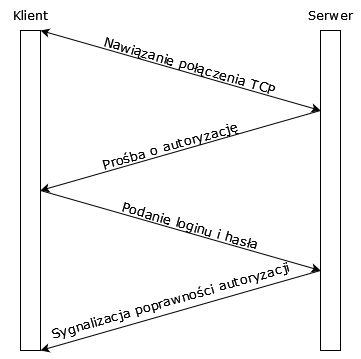
\includegraphics[width=0.6\textwidth]{img/auth.png}
\caption{\label{fig:auth.png}Schemat autoryzacji}
\end{figure}
\FloatBarrier
W przypadku niepomyślnej autoryzacji serwer wysyła do klienta ponowną prośbę o podanie danych. Po trzech nieudanych próbach serwer zamyka połączenie.

\subsection{Poruszanie się po katalogach}
Klient ma możliwość przejścia do katalogu domowego lub o jeden poziom względem bieżącego katalogu. Analogicznym działaniem w systemie Linux jest instrukcja \texttt{cd}.

\subsection{Wyświetlanie aktualnego katalogu}
Klient ma możliwość wyświetlenia ścieżki do aktualnego katalogu. Analogicznym działaniem w systemie Linux jest instrukcja \texttt{pwd}.

\subsection{Wypisywanie katalogów}
\noindent Istnieją dwie możliwości:
\begin{enumerate}
    \item Można wypisać wszystkie katalogi zaczynając od katalogu domowego (analogiczne polecenie systemowe to \texttt{tree}),
    \item Można wypisać podkatalogi i pliku znajdujące się w bieżącym katalogu (analogiczne polecenie systemowe \texttt{ls}).
\end{enumerate}

\subsection{Tworzenie katalogów}
Możliwe jest tworzenie katalogów tylko wewnątrz bieżącego katalogu, pojedynczo. Jeśli katalog o podanej nazwie już istnieje użytkownik otrzyma błąd.

Od momentu podania nazwy nowego katalogu jest ona już \quotes{zajęta}, w przypadku gdy dwie osoby spróbują stworzyć w tym samym czasie katalog o tej samej nazwie, jedna z nich otrzyma błąd.

\subsection{Tworzenie plików}
\begin{itemize}
    \item Scenariusz główny:
    \begin{enumerate}
        \item Klient wysyła do serwera żądanie utworzenia pliku o wskazanej nazwie w folderze, w którym obecnie się znajduje,
        \item Serwer sprawdza, czy w danym katalogu istnieje już plik o danej nazwie,
        \item Serwer tworzy plik o podanej nazwie w odpowiednim katalogu,
        \item Serwer wysyła do klienta potwierdzenie utworzenia nowego pliku.
    \end{enumerate}

    \item Scenariusz alternatywny -- próba utworzenia w \quotes{folderze klienta} pliku o tej samej nazwie co inny plik:
    \begin{enumerate}
        \item Kroki 1 -- 2 scenariusza głównego,
        \item Serwer wysyła do klienta odmowę wykonania operacji.
    \end{enumerate}
\end{itemize}

\subsection{Usuwanie plików i katalogów}
\begin{itemize}
    \item Scenariusz główny:
    \begin{enumerate}
        \item Klient wysyła do serwera żądanie usunięcia wskazanego pliku lub katalogu,
        \item Serwer sprawdza, czy istnieje katalog (lub plik) do usunięcia,
        \item Serwer sprawdza, czy w katalogu do usunięcia ktoś się znajduje lub czy plik do usunięcia jest aktualnie pobierany,
        \item Jeśli nie, to serwer usuwa katalog (lub plik) i wysyła potwierdzenie usunięcia do klienta.
    \end{enumerate}

    \item Scenariusz alternatywny I -- w katalogu do usunięcia ktoś się znajduje lub plik do usunięcia jest pobierany:
    \begin{enumerate}
        \item Kroki 1 -- 3 scenariusza głównego,
        \item Serwer wysyła do klienta odmowę wykonania operacji.
    \end{enumerate}

    \item Scenariusz alternatywny II -- próba usunięcia nieistniejącego pliku lub katalogu:
    \begin{enumerate}
        \item Kroki 1 -- 2 scenariusza głównego,
        \item Serwer wysyła do klienta odmowę wykonania operacji.
    \end{enumerate}
\end{itemize}

\subsection{Zmienianie nazwy plików i katalogów}
\begin{itemize}
    \item Scenariusz główny:
    \begin{enumerate}
        \item Klient wysyła do serwera żądanie zmiany nazwy pliku lub katalogu,
        \item Serwer sprawdza, czy istnieje plik lub katalog o tej samej nazwie w danym katalogu,
        \item Jeśli jest to plik, serwer sprawdza, czy jest on aktualnie pobierany,
        \item Jeśli jest to katalog, serwer sprawdza, czy aktualnie ktoś się w nim znajduje,
        \item Jeśli nie, serwer zmienia nazwę danego pliku lub katalogu i wysyła potwierdzenie do klienta.
    \end{enumerate}

    \item Scenariusz alternatywny I -- istnieje już plik lub katalog o tej samej nazwie:
    \begin{enumerate}
        \item Kroki 1 -- 2 scenariusza głównego,
        \item Serwer wysyła do klienta odmowę zmiany nazwy.
    \end{enumerate}

    \item Scenariusz alternatywny II -- próba zmiany nazwy pliku który jest obecnie pobierany:
    \begin{enumerate}
        \item Kroki 1 -- 3 scenariusza głównego,
        \item Serwer wysyła do klienta odmowę zmiany nazwy.
    \end{enumerate}

    \item Scenariusz alternatywny III -- próba zmiany nazwy katalogu w którym ktoś się znajduje:
    \begin{enumerate}
        \item Kroki 1 -- 4 scenariusza głównego,
        \item Serwer wysyła do klienta odmowę zmiany nazwy.
    \end{enumerate}
\end{itemize}

\subsection{Kopiowanie lub przenoszenie plików między katalogami}
\begin{itemize}
    \item Scenariusz główny:
    \begin{enumerate}
        \item Klient wysyła do serwera żądanie skopiowania pliku o danej nazwie do zadanego katalogu,
        \item Serwer sprawdza, czy istnieje katalog, do którego chcemy skopiować plik,
        \item Serwer sprawdza, czy w danym katalogu istnieje już plik o danej nazwie,
        \item Jeśli nie, serwer kopiuje plik do podanego katalogu.
    \end{enumerate}

    \item Scenariusz alternatywny I -- plik który chcemy skopiować jest w katalogu, w którym obecnie się nie znajdujemy:
    \begin{enumerate}
        \item Kroki 1  scenariusza głównego,
        \item Serwer wysyła do klienta odmowę skopiowania pliku.
    \end{enumerate}


    \item Scenariusz alternatywny II -- próba skopiowania pliku do katalogu, który nie istnieje:
    \begin{enumerate}
        \item Kroki 1 -- 2 scenariusza głównego,
        \item Serwer tworzy katalog o podanej nazwie, a następnie kopiuje do niego plik.
    \end{enumerate}

    \item Scenariusz alternatywny III -- próba skopiowania pliku w miejsce gdzie istnieje już inny o tej samej nazwie:
    \begin{enumerate}
        \item Kroki 1 -- 3 scenariusza głównego,
        \item Serwer wysyła do klienta odmowę skopiowania pliku.
    \end{enumerate}
\end{itemize}

\subsection{Pobieranie plików}
\noindent Klient może pobrać dany plik z serwera z aktualnego katalogu pod warunkiem, że ma do tego odpowiednie uprawnienia:
\begin{itemize}
    \item Scenariusz główny:
    \begin{enumerate}
        \item Klient wysyła pytanie o zgodę na pobranie pliku (\texttt{dl}). Zawiera się w niej przede wszystkim nazwa przesyłanego pliku,
        \item Serwer, po zweryfikowaniu uprawnień użytkownika, wysyła zgodę na pobieranie wraz z dodatkową informacją -- rozmiarem pliku,
        \item Klient wysyła komunikat inicjujący pobieranie (\texttt{dls}),
        \item Serwer przesyła dane strumieniowo do klienta, który musi odczytać dokładnie tyle bajtów ile zostało określone w odpowiedzi,
        \item Klient czyta bajty ze strumienia i dopisuje je do pliku o nazwie \quotes{\texttt{[NAZWA-ŁADOWANEGO-PLIKU].[SÓL].partial}} reprezentującego częściowo pobrane dane,
        \item Po przeczytaniu wszystkich bajtów aplikacja klienta zmienia nazwę pliku częściowego na docelową.
    \end{enumerate}

    \item Scenariusz alternatywny I - odmowa pobierania:
    \begin{enumerate}
        \item Krok 1 scenariusza głównego,
        \item Klient otrzymuje odmowę pobierania pliku (np. z powodu braku uprawnień) -- użytkownik dostaje informację o niepowodzeniu operacji.
    \end{enumerate}

    \item \textbf{Scenariusz alternatywny II -- przerwanie połączenia z siecią w trakcie pobierania pliku}:
    \begin{enumerate}
        \item Kroki 1 -- 4 scenariusza głównego,
        \item Przerwanie połączenia ze strony klienta lub serwera,
        \item Klient zapisuje do specjalnego pliku informację o przerwanej operacji. Zawiera się w niej ścieżka do pobieranego pliku, kod przerwanej operacji oraz numer pierwszego bajtu, który nie został odebrany,
        \item Klient i serwer oczekują na odzyskanie łączności z siecią,
        \item Klient nawiązuje ponownie połączenie z serwerem, loguje się na swoje konto,
        \item Klient sprawdza czy żadna operacja nie została wcześniej przerwana. Tak jest, zatem kieruje do użytkownika zapytanie o ponowienie operacji,
        \item Jeżeli użytkownik chce ponowić operację, to wykonywane są kroki 1 -- 2 scenariusza głównego,
        \item Klient wysyła komunikat ponawiający pobieranie (\texttt{dlr}). Zawiera on między innymi numer bajtu, od którego zacząć pobieranie,
        \item Serwer przesyła dokładnie $N - O$ bajtów, gdzie $N$ to rozmiar całego pliku (wysłany użytkownikowi we wcześniejszej odpowiedzi), a $O$ to number bajtu, od którego klient chce otrzymywać dane.
    \end{enumerate}
\end{itemize}

\subsection{Ładowanie plików}
\noindent Klient może załadować plik na serwer do aktualnego katalogu:
\begin{itemize}
    \item Scenariusz główny:
    \begin{enumerate}
        \item Klient wysyła pytanie o zgodę na załadowanie pliku. Zawiera się w niej między innymi nazwa przesyłanego pliku oraz jego rozmiar,
        \item Serwer, po zweryfikowaniu uprawnień użytkownika, wydaje zgodę na ładowanie wraz z dodatkowymi informacjami (np. jaki jest maksymalny możliwy rodzaj pojedynczego pakietu, kod identyfikujący operację),
        \item Klient nawiązuje dodatkowe połączenie TCP z serwerem, które będzie wykorzystywane do przesyłania danych,
        \item Klient dzieli plik na małe pakiety i wysyła je do serwera,
        \item Serwer odbiera fragmenty od klienta i dopisuje je do pliku o nazwie \quotes{\texttt{[NAZWA-ŁADOWANEGO-PLIKU].[SÓL].partial}} reprezentującego częściowo załadowane dane. Plik ten nie jest wyświetlany w przypadku żądania wypisania katalogu przez klienta,
        \item Ostatnim pakietem wysłanym przez klienta jest informacja o zakończeniu ładowania,
        \item Serwer zmienia nazwę pliku częściowego na docelową,
        \item Utworzone wcześniej dodatkowe połączenie TCP nie jest zamykane od razu -- istnieje możliwość wykorzystania go do kolejnych ładowań (lub pobrań).
    \end{enumerate}

    \item Scenariusz alternatywny I - odmowa ładowania:
    \begin{enumerate}
        \item Krok 1 scenariusza głównego,
        \item Klient otrzymuje odmowę ładowania pliku -- użytkownik dostaje informację o niepowodzeniu operacji.
    \end{enumerate}

    \item Scenariusz alternatywny II -- dodatkowe połączenie TCP z serwerem zostało wcześniej zestawione:
    \begin{enumerate}
        \item Kroki 1 -- 2 scenariusza głównego,
        \item Dodatkowe połączenie już istnieje -- serwer i klient będą je wykorzystywać do przesyłania danych,
        \item Kroki 4 -- 8 scenariusza głównego.
    \end{enumerate}

    \item Scenariusz alternatywny III -- dodatkowe połączenie TCP nie mogło zostać zestawione:
    \begin{enumerate}
        \item Kroki 1 -- 2 scenariusza głównego,
        \item Dodatkowe połączenie nie mogło zostać zestawione -- użytkownik dostaje informację o niepowodzeniu operacji.
    \end{enumerate}

    \item Scenariusz alternatywny IV -- klient wysłał nieprawidłowy fragment pliku:
    \begin{enumerate}
        \item Kroki 1 -- 4 scenariusza głównego,
        \item Klient wysłał nieprawidłowy fragment pliku -- serwer wysyła informację o błędzie i kończy operację. Nie zamyka on jednak zestawionego połączenia TCP -- może być wykorzystane później.
    \end{enumerate}

    \item \textbf{Scenariusz alternatywny V -- przerwanie połączenia z siecią w trakcie ładowania pliku}:
    \begin{enumerate}
        \item Kroki 1 -- 4 scenariusza głównego,
        \item Przerwanie połączenia ze strony klienta lub serwera,
        \item Serwer zapisuje do specjalnego pliku informację o przerwanej operacji. Zawiera się w niej między innymi nazwa użytkownika ładującego plik, kod operacji oraz ostatni odebrany fragment pliku,
        \item W tym samym czasie klient zapisuje do pliku informację o ostatnim wysłanym fragmencie pliku oraz lokalnej ścieżce do pliku,
        \item Klient i serwer oczekują na odzyskanie łączności z siecią,
        \item Klient nawiązuje ponownie połączenie z serwerem, loguje się na swoje konto,
        \item Klient sprawdza czy żadna operacja nie została wcześniej przerwana. Tak jest, zatem kieruje do użytkownika zapytanie o ponowienie operacji,
        \item Dwa możliwe scenariusze:
        \begin{itemize}
            \item Użytkownik ponawia ładowanie pliku:
            \begin{enumerate}
                \item Aplikacja klienta wysyła prośbę o ponowienie operacji ładowania,
                \item Serwer, po zweryfikowaniu że taka operacja faktycznie miała wcześniej miejsce, wyraża zgodę na ponowienie,
                \item Kroki 3 -- 8 scenariusza głównego.
            \end{enumerate}

            \item Użytkownik kończy operację ładowania pliku:
            \begin{enumerate}
                \item Aplikacja klienta wysyła informację o tym, że ładowanie nie będzie ponawiane,
                \item Serwer po otrzymaniu informacji usuwa wpis utworzony w punkcie 3 scenariusza alternatywnego V.
            \end{enumerate}
        \end{itemize}
    \end{enumerate}
\end{itemize}

\subsection{Struktura komunikatów}

\subsubsection{Komunikaty wysyłane przez klienta}
Każdy komunikat składa się z jednej linii, w której znajduje się nazwa polecenia oraz wielu linii w postaci \quotes{\texttt{nazwa\_pola:wartość}}. Wymagania:
\begin{enumerate}
    \item Kolejne komunikaty oddzielone są pustą linią (znak o kodzie \texttt{0x0A}),
    \item Każda linia może mieć maksymalnie długość 2048 bajtów. Po przeczytaniu tej ilości danych serwer zwróci błąd i rozpocznie analizę kolejnego polecenia,
    \item Każda polecenie może mieć maksymalnie 16 pól,
    \item Nazwa pola może składać się tylko z małych liter alfabetu łacińskiego,
    \item Między:
        \begin{itemize}
            \item Początkiem linii a nazwą pola,
            \item Nazwą pola a dwukropkiem,
            \item Dwukropkiem a wartością pola,
            \item Wartością pola a końcem linii,
        \end{itemize}
        Mogą znaleźć się białe znaki o kodach \texttt{0x09} (tabulacja) oraz \texttt{0x20} (spacja).
    \item Wartość pola może być typu:
        \begin{itemize}
            \item \texttt{boolean} -- pole jest typu logicznego, gdy jego wartość jest równa dokładnie \texttt{true} lub \texttt{false},
            \item \texttt{integer} -- pole jest typu całkowitego, gdy jego wartość składa się wyłączne z cyfr,
            \item \texttt{string} -- ostatecznie pole jest typu \texttt{string}. Jeżeli pierwszym i ostatnim znakiem pola jest apostrof (znak o kodzie \texttt{0x27}) to znaki te nie są brane pod uwagę przez interpreter (przykładowo wartość \quotes{\texttt{'value'}} jest tym samym co \quotes{\texttt{value}}).
        \end{itemize}
\end{enumerate}

\subsubsection{Odpowiedzi serwera}
\noindent Struktura odpowiedzi:
\begin{enumerate}
    \item Zawsze w pierwszej linii znajduje się kod zwrotny wykonanej operacji oraz nazwa wykonanego polecenie oddzielone spacją,
    \item Opcjonalnie w kolejnych liniach zawarte są szczegóły odpowiedzi. Struktura odpowiedzi zależy od kodu zwrotnego i wykonanej komendy,
    \item Odpowiedź jest zakończona pustą linią (znak o kodzie \texttt{0x0A}).
\end{enumerate}

\subsubsection{Kody zwrotne serwera}
\noindent Kod 100 (\texttt{ok}) oznacza, że żądana operacja powiodła się.
\noindent Kody błędów interpretera i wykonawcy komend:
\begin{itemize}
    \item \texttt{300 too\_long\_line} -- błąd ten oznacza, że przeczytana linia jest zbyt długa dla interpretera,
    \item \texttt{301 too\_many\_fields} -- błąd oznaczający, że klient podał zbyt wiele pól,
    \item \texttt{302 bad\_field} -- błąd oznaczający, że format pola jest nieprawidłowy (np. pole nie ma wartości),
    \item \texttt{303 bad\_command} -- błąd oznaczający, że wskazana komenda nie istnieje.
\end{itemize}
\noindent Kody błędów wykonywanych komend:
\begin{itemize}
    \item \texttt{401 unknown} -- nieznany błąd spowodowany np. poważnym błędem systemu operacyjnego serwera,
    \item \texttt{402 not\_logged\_in} -- błąd zwracany, gdy klient próbuje skorzystać z komendy wymagającej autoryzacji bez bycia zalogowanym (np. użycie \texttt{ls} przed komunikatem \texttt{auth}),
    \item \texttt{403 invalid\_field\_value} -- pole komunikatu ma nieprawidłową wartość lub jest nieprawidłowego typu,
    \item \texttt{404 not\_found} -- żądany obiekt nie został znaleziony (np. przy próbie  pobierania),
    \item \texttt{405 target\_not\_found} -- miejsce docelowe (np. przy kopiowaniu lub przenoszeniu) nie zostało znalezione,
    \item \texttt{406 not\_enough\_perms} -- użytkownik nie posiada uprawnień do wykonania danej operacji,
    \item \texttt{407 user\_already\_logged} -- błąd zwracany, gdy użytkownik próbuje użyć komunikatu \texttt{auth} będąc zalogowanym lub gdy inny użytkownik próbuje zalogować się na aktualnie używane konto,
    \item \texttt{408 invalid\_credentials} -- użytkownik próbuje użyć komunikatu \texttt{auth} z nieprawidłowymi danymi (np. zły login lub hasło).
\end{itemize}

\subsection{Polecenia}

% PRZYKŁAD
%
% NAZWA_POLECENIA
% POLE1: WARTOŚĆ1
% POLE2: WARTOŚĆ2
% POLE3: WARTOŚĆ3
% <--- PUSTA LINIA NA ZAKOŃCZENIE POLECENIA

\subsubsection{Polecenie \texttt{auth}}
Polecenie \texttt{auth} musi być pierwszym poleceniem wykonanym przez połączonego klienta -- bez poprawnej autoryzacji nie ma możliwości wykonywania jakichkolwiek innych komend. Dostępne pola:
\begin{itemize}
    \item \texttt{login} -- pole typu \texttt{string} zawierające nazwę użytkownika,
    \item \texttt{passwd} -- pole typu \texttt{string} zawierające hasło użytkownika.
\end{itemize}

\subsubsection{Polecenie \texttt{logout}}
Polecenie \texttt{logout} pozwala na wylogowanie się z aktualnego konta i przejście na np. inne.

\subsubsection{Polecenie \texttt{exit}}
Polecenie \texttt{exit} pozwala na bezpieczne rozłączenie się z serwerem. Jest to jedyne polecenie poza \texttt{auth}, które może być użyte bez logowania.

\subsubsection{Polecenie \texttt{cd}}
Polecenie \texttt{cd} służy do zmiany aktualnego katalogu użytkownika. Dostępne pola:
\begin{itemize}
    \item \texttt{path} -- pole typu \texttt{string} zawierające względną lub bezwzględną ścieżkę.
\end{itemize}
Polecenie to zwraca nową ścieżkę, o ile jego wykonanie się powiodło.

\subsubsection{Polecenie \texttt{name}}
Polecenie \texttt{name} zwraca nazwę użytkownika, na którego konto zalogowany jest klient.

\subsubsection{Polecenie \texttt{pwd}}
Polecenie \texttt{pwd} zwraca katalog, w którym aktualnie znajduje się użytkownik. Serwer w odpowiedzi w jednej linii zwróci ten katalog.

\subsubsection{Polecenie \texttt{ls}}
Polecenie \texttt{ls} zwraca listę plików dostępnych w danym katalogu. Dostępne pola:
\begin{itemize}
    \item \texttt{path} -- opcjonalne pole typu \texttt{string} zawierające ścieżkę do katalogu, którego pliki powinny zostać wypisane. Jeżeli pole to nie zostało określone to wykorzystany będzie aktualny katalog użytkownika,
    \item \texttt{size} -- opcjonalne pole typu \texttt{boolean}. Określa ono, czy użytkownik chce otrzymać w odpowiedzi rozmiary plików. Jeżeli serwer nie będzie w stanie pobrać rozmiaru to zwrócony zostanie znak \texttt{-} (kod ASCII \texttt{0x2D}),
    \item \texttt{mod} -- opcjonalne pole typu \texttt{boolean}. Określa ono, czy użytkownik chce otrzymać w odpowiedzi datę ostatniej modyfikacji plików w postaci \texttt{DD.MM.YYYY HH:MM:SS}. Jeżeli serwer nie będzie w stanie pobrać tej daty to zwrócony zostanie znak \texttt{-} (kod ASCII \texttt{0x2D}),
\end{itemize}
W odpowiedzi serwera w kolejnych liniach podane zostaną nazwy plików w cudzysłowach oraz dodatkowe parametry, w takiej kolejności jaka jest podana wyżej. Przykładowa odpowiedź serwera, gdy wszystkie pola opcjonalne mają wartość \texttt{true}:\\
\texttt{100 ls}\\
\texttt{"test.txt"\ 4096 "25.10.2021 09:24:14"} \\
\texttt{"test2.txt"\ 8192 "30.12.2020 13:23:10"} \\
\texttt{"directory"\ - "20.06.2019 20:55:09"}

\subsubsection{Polecenie \texttt{mkdir}}
Polecenie \texttt{mkdir} tworzy nowy katalog w aktualnym katalogu. Dostępne pola:
\begin{itemize}
    \item \texttt{name} -- pole typu \texttt{string} zawierające nazwę nowego katalogu.
\end{itemize}

\subsubsection{Polecenie \texttt{rm}}
Polecenie \texttt{rm} usuwa plik z aktualnego katalogu. Dostępne pola:
\begin{itemize}
    \item \texttt{name} -- pole typu \texttt{string} określające plik do usunięcia.
\end{itemize}

\subsubsection{Polecenie \texttt{rename}}
Polecenie \texttt{rename} zmienia nazwę określonego pliku znajdującego się w aktualnym katalogu Dostępne pola:
\begin{itemize}
    \item \texttt{oname} -- pole typu \texttt{string} określające nazwę pliku, którego nazwa będzie zmieniona,
    \item \texttt{nname} -- pole typu \texttt{string} zawierające nową nazwę.
\end{itemize}

\subsubsection{Polecenie \texttt{cp}}
Polecenie \texttt{cp} służy do kopiowania pliku z aktualnego katalogu w inne dostępne na serwerze miejsce. Dostępne pola:
\begin{itemize}
    \item \texttt{name} -- pole typu \texttt{string} określające nazwę pliku, który będzie kopiowany,
    \item \texttt{path} -- ścieżka do katalogu, w którym znajdzie się kopia pliku.
\end{itemize}

\subsubsection{Polecenie \texttt{mv}}
Polecenie \texttt{mv} służy do przenoszenia pliku z aktualnego katalogu w inne dostępne na serwerze miejsce. Dostępne pola:
\begin{itemize}
    \item \texttt{name} -- pole typu \texttt{string} określające nazwę pliku, który będzie przenoszony,
    \item \texttt{path} -- ścieżka do katalogu, w którym znajdzie się plik.
\end{itemize}

\subsubsection{Polecenie \texttt{dl}}

% dl
% name: <name>

% dls
% name: <name>

% dlr
% name: <name>
% offset: <offset> <--- kiedy skończyło się pobieranie

\subsubsection{Polecenie \texttt{ul}}

% ul
% name: <name>
% length: <length>

% uls
% name: <name>
% length: <length>
% <<<<pusta linia>>>>>
% DANE BINARNE

% CACHE: tylko ostatnie połączenie, kto ładował, co ładował, gdzie ładował i na jakim etapie skończył
% ulr
% name: <name>
% offset: <offset> <--- kiedy skończył się upload

\section{Serwer}

\subsection{Słownik pojęć}
\noindent Pojęcia używane w tej sekcji:
\begin{enumerate}
    \item TDS -- TinDox Server.
    \item Instancja serwera -- katalog zawierający katalog podrzędny o nazwie \texttt{.tds}, w którym znajdują pliki konfiguracyjne potrzebne do uruchomienia serwera. Instancja jest również korzeniem systemu plików widocznego przez klienta.
    \item IO - wejście i wyjście.
    \item Klient (\textit{Client}) -- każdy komputer podłączony do serwera.
    \item Użytkownik (\textit{User}) -- każdy wpisana nazwa na liście użytkowników.
\end{enumerate}

\subsection{Wymagania funkcjonalne}

\begin{enumerate}
    \item Możliwość szybkiego utworzenia instancji serwera w dowolnym miejscu na dysku.
    \item Tworzenie, modyfikacja i usuwanie użytkowników uprawnionych do korzystania z dysku sieciowego.
    \item Realizacja komunikacji z klientami z wykorzystaniem gniazd BSD.
    \item Wydajne IO dzięki wykorzystaniu zasobów systemowych:
    \begin{itemize}
        \item Wykorzystanie efektywnej liczby wątków do obsługi wielu klientów jednocześnie,
        \item Wykorzystanie linuksowego mechanizmu \texttt{epoll} do sprawnej obsługi aktywnych klientów.
    \end{itemize}
    \item Bezbłędne zamykanie połączeń z klientami oraz całego serwera.
    \item Prawidłowe reagowanie na sygnały systemowe (np. użycie \texttt{Ctrl+C} w terminalu powinno prawidłowo zakończyć działanie serwera).
    \item Monitorowanie połączeń przychodzących oraz błędów serwera, wypisywanie logów.
\end{enumerate}

\subsection{Wymagania niefunkcjonalne}

\begin{enumerate}
    \item Konfigurowalność -- serwer będzie wykorzystywał plik konfiguracyjny w formacie TOML. Edytując go, użytkownik będzie mógł dostosować serwer do możliwości swojego komputera, co oznacza między innymi:
    \begin{itemize}
        \item Możliwość wyboru maksymalnej ilości wątków używanych przez serwer (domyślnie będzie to wartość zwracana przez funkcję z języka \texttt{C++} -- \texttt{std::thread::hardware\_concurrency()}),
        \item Możliwość wyboru maksymalnej ilości klientów w sesji,
        \item Możliwość zmiany portu, na którym będzie nasłuchiwał serwer.
    \end{itemize}

    \item Wydajność -- serwer powinien sprawnie obsługiwać wiele żądań jednocześnie przy wykorzystaniu optymalnej ilości zasobów systemu operacyjnego.

    \item Bezpieczeństwo -- serwer powinien być odporny na złośliwe zapytania. Oznacza to, że w aplikacji nie wystąpią podatności takie jak np. \href{https://en.wikipedia.org/wiki/Arbitrary_code_execution}{RCE}.
\end{enumerate}

\subsection{Polecenia linii komend}

\subsubsection{Polecenie \texttt{help}}
Polecenie \texttt{help} służy do wyświetlenia pomocy, czyli między innymi listy dostępnych komend.

\subsubsection{Polecenie \texttt{init}}
Polecenie \texttt{init} służy do utworzenia instancji serwera, czyli katalogu \texttt{.tds} oraz innych istotnych plików konfiguracyjnych. Może być wywołane bez parametrów, wówczas instancja zostanie utworzona w bieżącym katalogu, lub z jednym argumentem, który jest ścieżką do istniejącego, docelowego folderu. Przykłady użycia:
\begin{itemize}
    \item \texttt{tds init} -- utworzenie instancji w bieżącym katalogu,
    \item \texttt{tds init .} -- to samo co wyżej,
    \item \texttt{tds init \$HOME} -- utworzenie instancji w katalogu domowym użytkownika.
\end{itemize}
Serwer zaraz po utworzeniu ma tylko jednego dostępnego użytkownika o nazwie \texttt{admin}, który posiada wszystkie dostępne uprawnienia.

\subsubsection{Polecenie \texttt{run}}
Polecenie \texttt{run} służy do uruchamiania serwera. Może być wywołane bez parametrów, wówczas serwer zostanie uruchomiony w bieżącym katalogu, o ile jest to prawidłowa instancja. Dodatkowo polecenie \texttt{init} definiuje dwie flagi:

\begin{itemize}
    \item \texttt{-{}-path [ścieżka]} -- wybór innej instancji serwera niż bieżąca,
    \item \texttt{-{}-port [port]} -- wybór innego portu (domyślnie port jest ładowany z pliku \texttt{config}).
\end{itemize}

\noindent Przykłady użycia:

\begin{itemize}
    \item \texttt{tds run} -- uruchomienie instancji serwera w bieżącym katalogu,
    \item \texttt{tds run -{}-path .} -- to samo co wyżej,
    \item \texttt{tds run -{}-port 80} -- uruchomienie instancji serwera na porcie 80,
    \item \texttt{tds run -{}-path \$HOME -{}-port 3000} -- uruchomienie instancji serwera w katalogu domowym użytkownika na porcie 3000.
\end{itemize}

\subsubsection{Polecenie \texttt{user}}
Polecenie \texttt{user} służy do tworzenia nowych użytkowników, zmiany ich haseł, usuwania ich oraz do dodawania i odbierania uprawnień. Przykłady:
\begin{itemize}
    \item \texttt{tds user add} -- rozpoczęcie dialogu, w trakcie którego zostaną podane login i hasło oraz powstanie nowy użytkownik,
    \item \texttt{tds user passwd admin} -- zmiana hasła użytkownika \texttt{admin} poprzez dialog,
    \item \texttt{tds user perms admin +u -d} -- zmiana uprawnień użytkownika \texttt{admin} -- od teraz może on ładować pliki na serwer, ale nie może ich pobierać. Lista liter odpowiadających uprawnieniom może być wyświetlona z wykorzystaniem instrukcji \texttt{tds help},
    \item \texttt{tds user remove admin} -- usunięcie użytkownika \texttt{admin}.
\end{itemize}

\subsubsection{Uprawnienia użytkowników}
\begin{itemize}
    \item \texttt{write}, \texttt{w} -- uprawnienie dające dostęp do komend modyfikujących strukturę plików, np. \texttt{mkdir}, \texttt{rm},
    \item \texttt{copy}, \texttt{c} -- uprawnienie dające dostęp do komendy kopiującej \texttt{cp},
    \item \texttt{copy}, \texttt{m} -- uprawnienie dające dostęp do komendy przenoszącej \texttt{mv},
    \item \texttt{download}, \texttt{d} -- uprawnienie dające dostęp do komend odpowiadających za pobieranie plików: \texttt{dl}, \texttt{dls}, \texttt{dlr},
    \item \texttt{upload}, \texttt{u} -- uprawnienie dające dostęp do komend odpowiadających za ładowanie plików: \texttt{ul}, \texttt{uls}, \texttt{ulr}.
\end{itemize}
Podstawowe komendy takie jak \texttt{cd}, \texttt{ls} czy \texttt{exit} nie wymagają uprawnień. Użytkownik zaraz po utworzeniu ma tylko uprawnienie do pobierania plików (\texttt{d}).

\subsection{Opis techniczny}

\subsubsection{Moduły}
\noindent Projekt składa się z następujących modułów:
\begin{enumerate}
    \item \texttt{cli} -- moduł odpowiadający za obsługę linii komend,
    \item \texttt{cli::user\_command} -- podmoduł odpowiadający za obsługę polecenia \texttt{tds user [...]},
    \item \texttt{command} -- moduł zawierający klasy służące do wykonywania poleceń użytkownika,
    \item \texttt{config} -- moduł odpowiadający za obsługę i tworzenie domyślnych plików konfiguracyjnych serwera,
    \item \texttt{ip} -- moduł udostępniający klasy i funkcje związane ze stosem sieciowym, np. abstrakcję adresów IP, obsługę gniazd,
    \item \texttt{linux} -- moduł udostępniający klasy i funkcje związane z systemem Linux, np. obsługę mechanizmu systemowego \texttt{epoll},
    \item \texttt{protocol} -- moduł odpowiadający za obsługę protokołu TinDox. Zawiera między innymi interpreter poleceń, obsługę błędów protokołu czy realizację modelu \quotes{Receiver--Sender},
    \item \texttt{protocol::execution} -- podmoduł zawierający klasy odpowiadające za wykonywanie i odpowiadanie na polecenia klienta,
    \item \texttt{server} -- moduł zawierający klasy najwyższego poziomu odpowiadające za prawidłową komunikację między pozostałymi modułami,
    \item \texttt{user} -- moduł odpowiadający za parametry użytkowników serwera, czyli np. uprawnienia.
\end{enumerate}

\subsection{Narzędzia i biblioteki}

\subsubsection{Narzędzia}
\bgroup
    \begin{center}
        \def\arraystretch{1.3}
        \begin{tabular}{c|c|c}
            \textbf{Element} & \textbf{Narzędzia} & \textbf{Wersja} \\
            \hline
            Język programowania & \texttt{C++} & ISO/IEC 14882:2020 \\
            \hline
            Kompilator & \makecell{\texttt{g++} \\ \texttt{clang}} & \makecell{11.1.0 \\ 13.0.0} \\
            \hline
            System budowania & \texttt{\href{https://cmake.org/}{CMake}} & \makecell{3.18.4} \\
            \hline
            Automatyzacja testów & \texttt{CTest} & \makecell{3.18.4} \\
            \hline
            Platforma docelowa & \texttt{Linux x86-64} & \makecell{4.0 \\ 5.13}
        \end{tabular}
    \end{center}
\egroup

\subsubsection{Biblioteki}
\bgroup
    \begin{center}
        \def\arraystretch{1.3}
        \begin{tabular}{c|c|c}
            \textbf{Nazwa} & \textbf{Wersja} & \textbf{Opis} \\
            \hline
            \texttt{\href{https://github.com/catchorg/Catch2}{Catch2}} & 3.0.0 & Tworzenie testów jednostkowych \\
            \hline
            \texttt{\href{https://github.com/marzer/tomlplusplus}{tomlplusplus}} & 2.5.0 & Obsługa formatu TOML \\
            \hline
            \texttt{\href{https://github.com/fmtlib/fmt}{\{fmt\}}} & 8.0 & \makecell{Formatownie tekstów \\ Implementacja \texttt{std::format} (\texttt{C++20})} \\
            \hline
            \texttt{\href{https://github.com/gabime/spdlog}{spdlog}} & 1.9 & Tworzenie logów \\
        \end{tabular}
    \end{center}
\egroup

\section{Klient mobilny}

\subsection{Opis klienta}
Połączenie z serwerem za pomocą klienta w aplikacji mobilnej zaimplementowane z użyciem języka kotlin w środowisku Android Studio. Za ich pomocą powstanie prosta aplikacja mobilna z interakcyjnym interfejsem graficznym reprezentująca nasz zdalny system plików. Aplikacja będzie budowana na system Android.

\subsection{Narzędzia i biblioteki}
\bgroup
    \begin{center}
        \def\arraystretch{1.3}
        \begin{tabular}{c|c}
            \textbf{Element} & \textbf{Narzędzia} \\
            \hline
            Język programowania & \texttt{Kotlin} \\
            \hline
            Kompilator & \texttt{kotlinc} \\
            \hline
            IDE & \texttt{Android Studio} \\
            \hline
            Platforma docelowa & \texttt{Android}
        \end{tabular}
    \end{center}
\egroup

\section{Klient okienkowy}

\subsection{Opis klienta}
Połączenie z serwerem realizowane przez klienta okienkowego zaimplementowanego z użyciem języka Java i klasy Socket, która reprezentuje gniazda klienckie. Po uruchomieniu klient podejmie próbę połączenia z serwerem. W przypadku udanego połączenia aplikacja umożliwi interakcję ze zdalnym systemem plików.

\subsection{Narzędzia i biblioteki}
\bgroup
    \begin{center}
        \def\arraystretch{1.3}
        \begin{tabular}{c|c}
            \textbf{Element} & \textbf{  Narzędzia  } \\
            \hline
            Język programowania & \texttt{Java}  \\
            \hline
            Kompilator & \texttt{javac} \\
            \hline
            Testy jednostkowe & \texttt{JUnit}  \\
            \hline
            System budowania & \texttt{Gradle}  \\
        \end{tabular}
    \end{center}
\egroup

\section{Klient konsolowy}

\subsection{Opis klienta}
Połączenie z serwerem realizowane poprzez klienta zaimplementowanego przy użyciu biblioteki \texttt{ncurses} i języka \texttt{C}. Ncurses to zbiór funkcji i narzędzi pozwalających tworzyć zgrabne TUI. Wykorzystując elementy biblioteki powstanie narzędzie do wykonywania operacji plikowych na zdalnym systemie plików.

Klient konsolowy przeznaczony jest na system \texttt{Ubuntu}. Będzie kompilowany z wykorzystaniem \texttt{gcc} oraz budowany z wykorzystaniem \texttt{CMake}.

\subsection{Narzędzia i biblioteki}

\bgroup
    \begin{center}
        \def\arraystretch{1.3}
        \begin{tabular}{c|c|c}
            \textbf{Element} & \textbf{Narzędzia} & \textbf{Wersja} \\
            \hline
            Język programowania & \texttt{C++} & ISO/IEC 14882:2020 \\
            \hline
            Kompilator & \makecell{\texttt{g++}} & \makecell{11.2.0} \\
            \hline
            System budowania & \texttt{\href{https://cmake.org/}{CMake}} & \makecell{3.22.0} \\
            \hline
            TUI & \texttt{ncurses} & 6.2 \\
            \hline
            Platforma docelowa & \texttt{Linux x86-64} & 4.0.0
        \end{tabular}
    \end{center}
\egroup

\section{Metody testowania}

\begin{enumerate}
    \item Testy jednostkowe -- testowanie najważniejszych modułów poszczególnych projektów (np. modułu raportującego w serwerze lub składowych konstrukcji MVC w aplikacji mobilnej).
    \item Testy integracyjne -- testy weryfikujące poprawność komunikacji między największymi składnikami całego systemu (np. między klientem konsolowym a serwerem).
    \item \textit{Fuzzing} -- automatyczne testowanie reakcji serwera na losowe wiadomości przychodzące od klienta.
    \item Testy obciążeniowe -- zautomatyzowane testowanie wytrzymałości serwera na zapytania przychodzące od dużych ilości klientów.
    \item Testy penetracyjne -- testy wykonywane w celu znalezienia podatności w oprogramowaniu serwera oraz klientów.
    \item Testy empiryczne -- testy wykonywane w czasie prezentacji programów dowodzące poprawności ich działania.
\end{enumerate}

\section{Zespół}

\subsection{Środowisko deweloperskie}

\bgroup
    \begin{center}
        \def\arraystretch{1.3}
        \begin{tabular}{c|c|c}
            \textbf{Element} & \textbf{Narzędzia} & \textbf{Wersja} \\
            \hline
            System operacyjny & \texttt{\makecell{Ubuntu \\ Manjaro Linux \\ Windows \\ Arch Linux}} & \makecell{20.04, 21.10 \\ 21.1.6 \\ 10.0 \\ ---} \\
            \hline
            \makecell{Pomocniczy język \\ skryptowy\footnotemark[1]} & \texttt{\makecell{Python \\ Bash}} & \makecell{3.9.7 \\ 5.1.8} \\
            \hline
            Kontrola wersji & \texttt{git} & 2.32.0 \\
            \hline
            \makecell{Repozytorium \\ ITS\footnotemark[2] \\ Tablica kanban} & \texttt{\makecell{\href{https://github.com/JMazurkiewicz/TIN-project}{GitHub} \\ \href{https://github.com/JMazurkiewicz/TinDox/issues}{GitHub Issues} \\ \href{https://github.com/JMazurkiewicz/TinDox/projects/1}{GitHub Projects}}} & --- \\
            \hline
            CI/CD & \texttt{Github Actions} & --- \\
            \hline
            Dokumentacja & \texttt{\href{https://www.overleaf.com/read/knbjwfrmvhzq}{Overleaf}} & --- \\
        \end{tabular}
    \end{center}
\egroup
\footnotetext[1]{Języki skryptowe będą używane do np. symulowania złożonych przypadków testowych, automatyzacji testów.}
\footnotetext[2]{Issue tracking system.}

\subsection{Podział pracy}

\begin{center}
    \begin{tabular}{l|r}
        \textbf{Projekt} & \textbf{Wykonawca} \\
        \hline
        Serwer & Jakub Mazurkiewicz \\
        Klient mobilny & Damian Piotrowski \\
        Klient okienkowy & Anna Pyrka \\
        Klient konsolowy & Łukasz Reszka
    \end{tabular}
\end{center}

\end{document}
